


Tal y como hemos mencionado en la introducción a este capítulo, los
conjuntos forman la base de las matemáticas. TKTK.





\subsubsection{Definición de \emph{conjunto}}

Aunque tenga una idea de qué quiere decir la palabra \emph{conjunto}
(\emph{set}), tanto por su uso en la lengua cotidiana como por nociones de
cursos anteriores de matemáticas que haya seguido, en realidad es un
concepto bastante difícil de definir.

Debido a esto, lo que se suele hacer es presentarlo de forma intuitiva, cosa
que en los textos de matemáticas muchas veces califican de ``ingenua''
(\emph{naive} o \emph{naïve}). Así, el estudiante queda satisfecho al
conocer lo básico sobre qué es un conjunto y cómo se comporta, y puede
dedicarse a hacer un uso práctico de este tipo de objetos matemáticos; que
es lo que interesa la mayoría de las veces, en lugar de hacer deliberaciones
sobre cómo se podría definir formalmente ese tipo de objetos.

% TODO Quizás, pasarlo al comienzo del texto.

Además, es bastante común que los textos de matemáticas de nivel
universitario tengan apéndices donde se expone lo básico sobre lógica y
teoría de conjuntos, así como algunos otros conceptos que se tratan aquí. En
esta asignatura, se tratan en bastante mayor detalle TKTK.

\begin{deffinition}[Conjunto (``ingenua'')]
  Un conjunto es una colección de objetos.
\end{deffinition}

\noindent ¿Pero qué es una \emph{colección}? En realidad, quiere decir lo
mismo que \emph{conjunto}, con lo que estaríamos usando en la definición la
palabra a definir, cosa que está prohibida\dots{} aunque no siempre lo está,
tal y como veremos más adelante. En cualquier caso, para esta definición no
tiene sentido usar la autoreferencia y se usa simplemente para que el lector
se quede satisfecho. Una definición real de este término es mucho más
compleja y extensa, y aquí solo se verá por encima, en la sección de
comentarios.

Quédese, por tanto, con esta definición ``ingenua'', o, si lo prefiere tome
al concepto de \emph{conjunto} como sinónimo de \emph{colección},
\emph{falimia}, \emph{agrupación}, etc., sobre los que también tendrá casi
con toda seguridad una idea intuitiva.

Un conjunto lo pueden constituir, por ejemplo, las letras del abecedario de
la lengua española. Otro, los meses del año. Etc.

Los conjuntos se suelen designar mediante letras mayúsculas del alfabeto
latino, o, a veces, de otros alfabetos, como, por ejemplo, el griego: $A$,
$B$, $X$, $\Omega$, etc.

Tan interesante como lo que se dice en la definición es lo que no se dice.
Es decir, se trata de un concepto muy amplio, con pocas limitaciones. Por un
lado, ya que no se especifica lo contrario, no nos interesa la naturaleza de
esos objetos. Existirán, por tanto, conjuntos de objetos de cualquier tipo,
permitiendo la heterogeneidad, es decir, en un conjunto pueden aparecer
objetos que se clasificarían naturalmente como de agrupaciones distintas,
pero eso da igual; pueden aparecer como se desee.

Además, un objeto puede estar en varios conjuntos simultáneamente. También,
nada impide que los objetos del conjunto sean conjuntos a su vez. Bueno, en
realidad, sobre esta última propiedad sí se debería puntualizar algo, pero
eso lo veremos luego.

A esos objetos que constituyen los conjuntos, en la terminología matemática
se les conoce como \semph{elementos} (\emph{elements}). Los elementos se
suelen designar mediante letras minúsculas del alfabeto latino, o, a veces,
de otros alfabetos, como, por ejemplo, el griego: $a$, $b$, $x$, $\omega$,
etc.





\subsubsection{Pertenencia}

A este respecto, existe una propiedad sobre las distintas entidades. Se
puede ver si una entidad es un elemento de un conjunto o si, por el
contrario, no lo es. Esta propiedad se conoce como la \emph{relación de
pertenencia}.\footnotemark

\footnotetext{Ahora, me doy cuenta de que estoy usando una terminología
demasiado rigurosa. Podemos hablar de \emph{elementos} en forma general,
como una entidad. Aunque se trate de una entidad que no pertenezca a ningún
conjunto, hablaremos de elementos. En realidad, cualquier entidad siempre
pertenecerá al menos a un conjunto: el conjunto formado por ese elemento. No
es ninguna trampa: puedo crear conjuntos a mi antojo. TKTK.}

Siguiendo con la pertenencia, que un elemento $a$ pertenezca a un conjunto
$C$ se expresa en notación simbólica como

$$ a \in C $$

\noindent cosa que se expresaría verbalmente como ``$a$ pertenece a $C$'',
``$a$ es un elemento de $C$'' o, también, ``$C$ contiene al elemento $a$''.
Por el contrario, si dicha proposición es falsa, será cierta la proposición
negación de esta, es decir, ``$a$ no pertenece a $C$'', ``$a$ no es un
elemento de $C$'' o, también, ``$C$ no contiene al elemento $a$'', y se
designaría por ``$a \notin C$''.

Un conjunto está \emph{bien definido} cuando no existe ambigüedad en la
relación de pertenencia, para ningún elemento. Es decir, cuando se tiene un
criterio que permite decidir si un elemento cualquiera pertenece o no a
dicho conjunto. Una expresión como ``el elemento $b$ pertenece al conjunto
$C$'' la interpretaremos como una proposición, como las que vimos en el
capítulo anterior, ya que se trata de un enunciado al que podemos atribuir
un valor lógico.

Aunque quizás en este momento no se le ocurra ningún caso en el que se diese
esa ambigüedad, estrujando un poco el ingenio, tal y como veremos más
adelante, puede que existan ``conjuntos'' para los que no podemos hacer esa
afirmación. Esas agrupaciones no las consideraremos conjuntos. Se trataría
de las paradojas de la teoría de conjuntos. Estas paradojas motivaron el
esfuerzo de crear una teoría de conjuntos más complicada con una base
sólida.

\begin{example}\label{ejemplo:conjuntos_01}
  Veamos algunos ejemplos de conjuntos:

  \begin{enumerate}
    \item Los números 1 y 2.
    \item Las soluciones enteras de la ecuación $x^2 - 3x + 2 = 0$.
    \item Los países de Europa en el año 2010.
    \item Las letras del abecedario.
    \item Los números pares.
    \item Las vocales del abecedario del español.
    \item El conjunto formado por el número 2, la vocal \emph{i}, y el museo
      del Prado.
  \end{enumerate}
\end{example}





\subsubsection{Igualdad}

Se dice que dos conjuntos $A$ y $C$ son \semph{iguales}, y se escribe $A =
C$, si y solo si tienen los mismos elementos. En caso contrario, se dice que
$A$ y $C$ son \emph{distintos} y se escribe $A \neq C$.

En el ejemplo anterior, los conjuntos dados en los puntos 1, 6 y 7 están
expresados (o definidos, también se dice) dando una lista de sus elementos.
Cuando expresamos un conjunto mediante una lista de todos sus elementos, se
dice que se ha expresado \semph{por extensión}. En notación simbólica, se
hace poniendo la lista de elementos, separados entre sí por comas,
``envolviéndolos'' entre signos de llaves. Las expresiones

\[
  \begin{array}{ccc}
    A = \{1, 2\}
      & B = \{a, e, i, o, u\}
      & C = \{2, i, \text{museo del Prado}\}
  \end{array}
\]

\noindent corresponden a los conjuntos de los puntos 1, 6 y 7 del ejemplo
anterior.

Algo que debe saber también sobre los conjuntos es que no se tiene en cuenta
el orden de los elementos ni la multiplicidad de apariciones de estos, ya
que en la definición no se especifica lo contrario. Como ve, los conjuntos
son unos objetos muy básicos. Así, si

$$
\begin{array}{lcr}
  A = \{1, 2\}
    & D = \{1, 1, 2\}
    & E = \{2, 1\}
\end{array}
$$

\noindent se tiene entonces que $A = D = E$, es decir, se trata del mismo
conjunto. Los elementos son los mismos aunque en el conjunto $D$ el elemento
1 se haya escrito dos veces y en $E$ se haya alterado el orden de los
elementos respecto a $A$. Se suele seguir la norma de expresar los conjuntos
de la forma más breve posible, con lo que no es normal que vea un conjunto
expresado por extensión en el que aparece un elemento
repetido.\footnotemark{} En cuanto al orden, aunque tampoco se tiene en
cuenta, lo normal es, por claridad, si existe cierto orden natural para sus
elementos, presentar a estos siguiéndolo; pero no olvide nunca que eso es
simplemente una regla de estilo que no indica nada en lógica ni en
matemáticas. Así, por ejemplo, si se trata el conjunto de los números pares,
se pondrán normalmente en el orden que ve a continuación:

\footnotetext{A este respecto, quizás le interese saber que existe una clase
de objetos en matemáticas que son como los conjuntos pero en los que sí se
tiene en cuenta la multiplicidad de apariciones de los elementos. Estos son
los multiconjuntos (\emph{multisets}), pero no los trataremos en esta
asignatura. Tienen su utilidad en combinatoria.}

$$ A = \{2, 4, 6, 8, 10, 12, \dots\} $$

\noindent Por cierto, es muy común hacer uso de puntos
suspensivos\footnotemark, `$\dots$', para expresar por extensión conjuntos
que no terminan nunca. Es el caso del conjunto $A$ anterior. A la vista de
los primeros elementos, en el orden en el que se disponen, el lector debería
saber intuir cómo serían los demás. No es una forma rigurosa de expresar el
conjunto, pero se usa bastante en la práctica. La otra forma de expresar un
conjunto, distinta a por extensión, permite expresar sin ambigüedad
conjuntos ilimitados, pero la veremos más adelante.

\footnotetext{también se le conoce como \emph{elipsis} (\emph{ellipsis})
TKTK}

Dado un elemento cualquiera $a$, se considera el conjunto cuyo único
elemento es $a$. A este lo denotaremos por $\{a\}$ y se dice que es un
\semph{conjunto unitario} (\emph{singleton}). Advierta que $a \in \{a\}$ y,
además, que las expresiones $a$ y $\{a\}$ indican cosas distintas: la
primera no tiene por qué ser un conjunto (aunque podría serlo), pero sí la
segunda.





\subsubsection{Inclusión}

Dados dos conjuntos $A$ y $B$, se dice que ``$B$ está incluido en $A$'' si y
solo si cualquier elemento del conjunto $B$ es un elemento del conjunto $A$.
De forma simbólica, esta relación de inclusión la denotaremos con la
expresión

$$ B \subseteq A $$

\noindent En este caso, se dice también que ``$B$ es un subconjunto de $A$''
o que ``$B$ está contenido o incluido en $A$''. La escritura equivalente $A
\supseteq B$ se lee como ``$A$ contiene a $B$'', o cualquiera de las
alternativas como ``$B$ está incluido en $A$'', que expresa lo mismo que $B
\subseteq A$.

Esta relación suele recibir el nombre de \emph{inclusión} o
\emph{contención} de conjuntos.

Si no se cumple la inclusión, se escribirá $B \not\subseteq A$.

A este respecto, la terminología puede variar en los distintos textos. TKTK.
En muchos textos encontrará que se usa el símbolo `$\subset$', en lugar de
`$\subseteq$'. TKTK. No inclusión. TKTK. Subconjunto propio. TKTK.

Ejemplo. El conjunto de los días del fin de semana es un subconjunto del
conjunto de los días de la semana:

$$ \{\text{sábado}, \text{domingo}\} \subseteq \{\text{lunes},
\text{martes}, \text{miércoles}, \text{jueves}, \text{viernes},
\text{sábado}, \text{domingo}\} $$

El conjunto de los números naturales que son potencia de 2 es un subconjunto
del conjunto de los números naturales pares. Tal y como verá más adelante,
en esta asignatura iremos aprendiendo a usar la simbología y así expresar de
forma breve y precisa un enunciado como este último.

Dados dos conjuntos $A$ y $B$, claramente se cumple

$$ A = B \ \text{si y solo si} \ A \subseteq B \ \text{y} \ B \subseteq A $$

\noindent Esta es la forma en la que demostramos en la práctica la igualdad
de dos conjuntos. La solemos llamar ``la doble inclusión''.

Una manera sencilla de representar la inclusión o la pertenencia en los
conjuntos se hace mediante los llamados diagramas de Venn. En ellos, se
representa cada conjunto mediante un círculo, un óvalo o cualquier área
cerrada en el plano. La posición relativa en el plano entre los círculos
muestra la inclusión entre conjuntos. En la
figura~\ref{fig:diagramas-venn-1}, se representa el conjunto $A = \{a, b, c,
d, e\}$ y, en la~\ref{fig:diagramas-venn-2}, los conjuntos $B = \{a, b, d\}$
y $A$, donde puede comprobar que se da la ralación $B \subseteq A$.

\begin{figure}
  \centering
  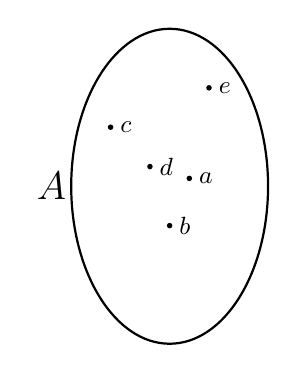
\begin{tikzpicture}[scale=0.5]
    % Dibujar el conjunto A como una elipse
    \draw[thick] (0,0) ellipse (2.5cm and 4cm);

    % Etiqueta del conjunto
    \node at (-3, 0) {\Large $A$};

    % Puntos dentro del conjunto
    \fill (-1.5, 1.5) circle (2pt) node[right] {\small $c$};
    \fill (-0.5, 0.5) circle (2pt) node[right] {\small $d$};
    \fill (0.5, 0.2) circle (2pt) node[right] {\small $a$};
    \fill (0, -1) circle (2pt) node[right] {\small $b$};
    \fill (1, 2.5) circle (2pt) node[right] {\small $e$};

  \end{tikzpicture}
  \caption{Diagrama de Venn de $A$}%
  \label{fig:diagramas-venn-1}
\end{figure}

\begin{figure}
  \centering
  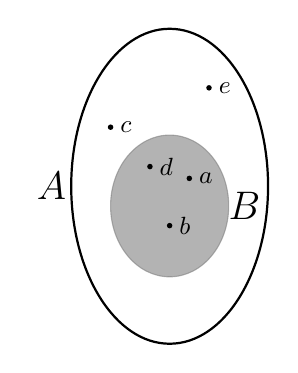
\begin{tikzpicture}[scale=0.5]
    % Dibujar el conjunto A como una elipse
    \draw[thick] (0,0) ellipse (2.5cm and 4cm);

    % Etiqueta del conjunto A
    \node at (-3, 0) {\Large $A$};

    % Dibujar el conjunto B como un círculo más pequeño dentro de A
    \filldraw[opacity=0.6, black!50] (0, -0.5) ellipse (1.5cm and 1.8cm);

    \fill (-1.5, 1.5) circle (2pt) node[right] {\small $c$};
    \fill (-0.5, 0.5) circle (2pt) node[right] {\small $d$};
    \fill (0.5, 0.2) circle (2pt) node[right] {\small $a$};
    \fill (0, -1) circle (2pt) node[right] {\small $b$};
    \fill (1, 2.5) circle (2pt) node[right] {\small $e$};

    % Etiqueta del conjunto B
    \node at (1.9, -0.5) {\Large $B$};
  \end{tikzpicture}
  \caption{Diagrama de Venn de $B \subseteq A$}%
  \label{fig:diagramas-venn-2}
\end{figure}

Algo que debe saber es que la inclusión de conjuntos cumple la propiedad
transitiva. Es decir, dados 3 conjuntos $A$, $B$, $C$, si se dan $A
\subseteq B$ y $B \subseteq C$, entonces se dará $A \subseteq C$. TKTK.



